\chapter{Projektbeskrivelse}

\section{Projektgennemførelse}
Ud fra den givne projektformulering og tilgang til emnet er der udformet en tidsplan, som indeholder de overordnede deadlines for review og tests givet fra AU.
\begin{figure}[H]
	\centering
	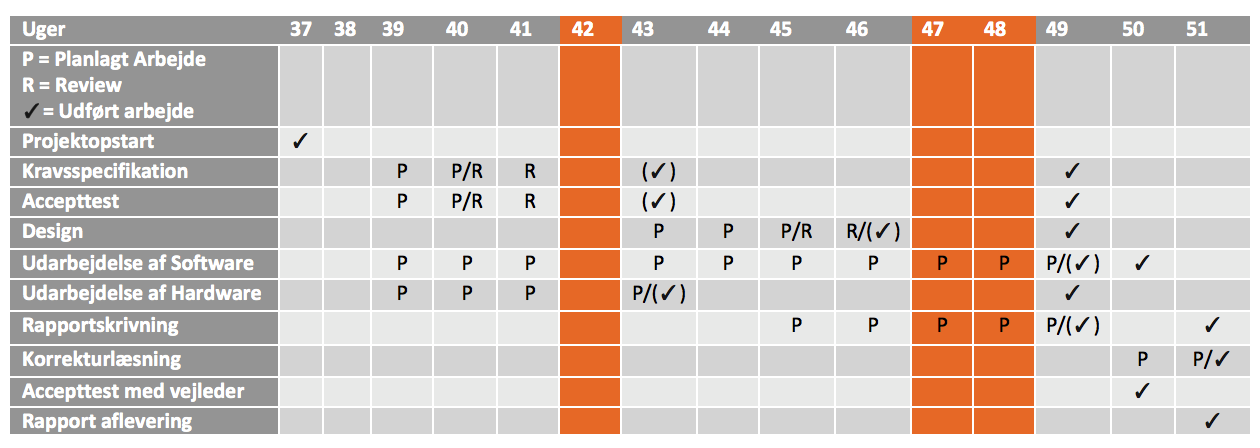
\includegraphics[width=1\textwidth]{Figurer/Snip20151210_74.png}
	\caption{Overordnet tidsplan}
\end{figure}
Udviklingsprocessen, Scrum, er blandt andet blevet brugt i nedbrydning af selve opgaven i delelementer, hvor de vigtigste delopgaver er prioriteret først. Via Scrum inddeles arbejdet i sprints, hvilket tidsplanen ligeledes er blevet. Sprints er forskellige faser, som eksempelvis projektopstart, kravspecifikation, accepttest, design osv.\\\\
I tidsplanen er der markeret et P for det planlagte arbejde, hvor reviews er markeret med bogstavet R. Derudover er der markeret flueben i tidsplanen for udført arbejde. Flueben i parentes repræsenterer, hvornår arbejdet skulle have været færdig, men ikke blev det. Uge 42 er markeret med orange farve, da der var efterårsferie, og her var der heller ikke planlagt arbejde. Uge 47 og 48 er også markeret med orange farve og bogstavet P, da der i denne periode har været planlagt arbejde. Dette arbejde er dog ikke blevet udført grundet eksamenslæsning og eksamen.
\\\\
\\\\
\\\\
\subsection{Deadlines}
Der er fra projektets start blevet stillet deadlines til forskellige dele af projektet.

\begin{longtabu} to \linewidth{@{}l X[j]@{}}
	Dato &    Deadlines \\[-1ex]
	\midrule
	02.10.2015		&	Aflevering af kravspecifikation og accepttest til review-gruppen \\[-1ex]
	09.10.2015			&	Review af kravspecifikation og accepttest færdiggjort med review-gruppen\\[-1ex]
	06.11.2015		&	Aflevering af design til review-gruppen \\[-1ex]	
	13.11.2015		&	Review af design færdiggjort med review-gruppen \\[-1ex] 
	11.12.2015		&	Accepttest med vejleder\\[-1ex]
	16.12.2015		&	Aflevering af projekt\\[-1ex]
	\caption{Deadlines}
\end{longtabu}
De første to deadlines i Tabel 6.1 har omhandlet kravspecifikation og accepttesten, hvor kravspecifikation er blevet udarbejdet først, efterfulgt af accepttesten. Derudover har der været deadlines til design, samt accepttest med vejleder og projektaflevering. 

\subsection{Mødestruktur}
Der er blevet fastlagt mødestruktur ved projektets start, hvor alle gruppens medlemmer har udarbejdet en samarbejdsaftale. Et ugentligt møde med vejleder efterfulgt af gruppemøde er blevet afholdt hver onsdag. Derudover er der blevet holdt gruppearbejde/gruppemøde efter behov. Hvert møde er blevet indledt med en opsamling af projektet samt dagsorden. Facebook er blevet brugt til komminukation omkring møder, samt en fælles kalender over iCloud. \\\\ Der er blevet ført logbog for samtlige møder med vejleder, samt logbog ved møder gruppermedlemmerne imellem.

\subsection{ASE-modellen}
Projektets udviklingsproces har taget udgangspunkt i ASE-modellen, som ses på nedenstående figur. Denne afspejles desuden også i den overordnede tidsplan. 
\begin{figure}[H]
	\centering
	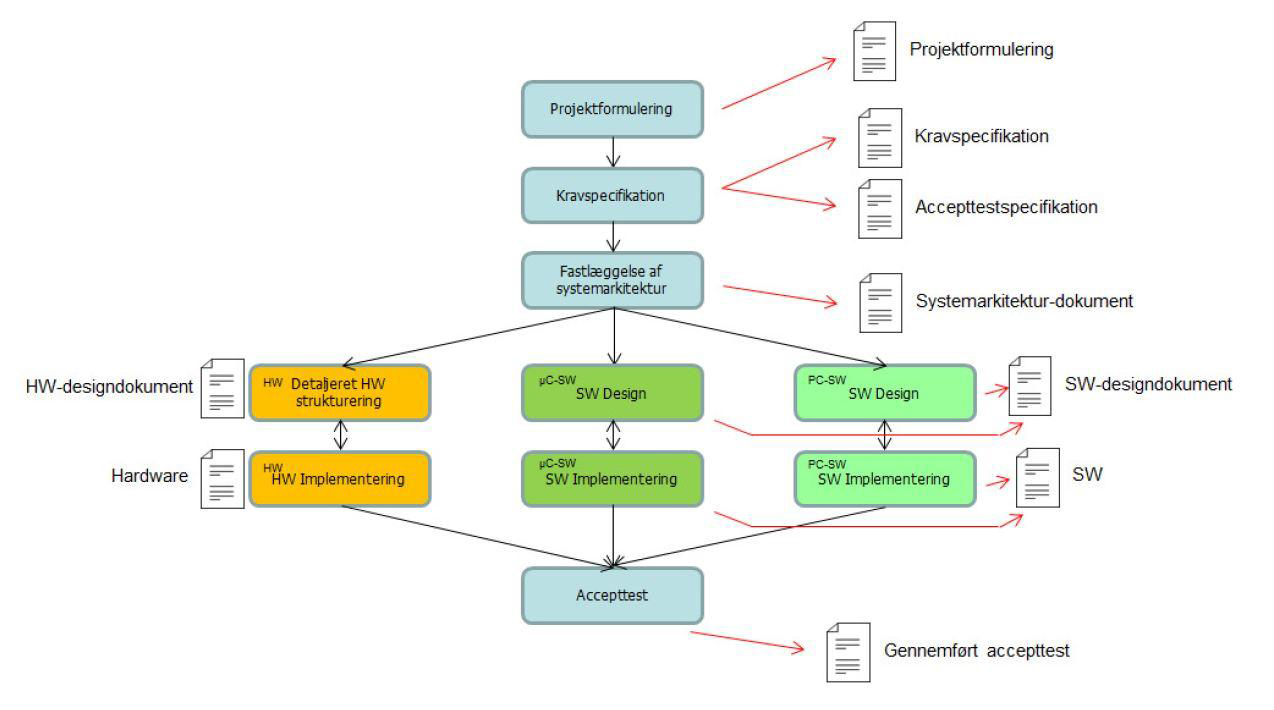
\includegraphics[width=1\textwidth]{Figurer/asemodel}
	\caption{Udviklingsmodel: ASE-model}
\end{figure}
ASE-modellen er en udviklingsmodel, der tager udgangspunkt i use cases, som defineres i kravspecifikationen i starten af projektarbejdet. ASE-modellen er inspireret af vandfaldsmodellen, hvor projektarbejdet opdeles i faser. Der fastlægges en opgaveformulering, kravspecifikation og systemarkitektur, for derefter at designe, implementere og teste de enkelte moduler i iterationer. Ud fra projektformuleringen specificeres kravspecifikationen som en række use cases, der beskriver de forskellige aktørers interaktion med systemet. Dette giver et overblik over, hvilke krav, der stilles til systemets funktionalitet. Ud fra kravspecifikationen bliver systemets accepttest udarbejdet. Efter kravspecifikationen er fastlagt, udarbejdes systemarkitekturen. Ud fra systemarkitekturen designes systemet ved at nedbryde det efter funktionalitet, som kan bindes til både software og hardware. \\\\
De første step i udviklingen af projektet iflg. ASE-modellen er blevet udarbejdet af alle gruppens medlemmer. Alle har bidraget til projektformuleringen, kravspecifikationen og accepttesten. I begyndelsen var der primært fokus på, at få dette færdiggjort, men der blev allerede her arbejdet på komponentværdier og udkast til hardwaren. I starten af projektarbejdet var det udtænkt, at alle gruppens medlemmer skulle arbejde med alle områder i projektet. Dette kunne ikke udføres rent tidsmæssigt, og derfor var en opdeling af arbejdsopgaver i mindre grupper nødvendig. Det blev delt op i software- og hardwarehold, dog var en del af hardwaren allerede beregnet og implementeret, da denne opdeling fandt sted. Tilbage af hardwaredelen var at lodde det på et veroboard og derefter teste det.\\\\

\subsection{V-modellen}
V-modellen er en udviklingsmodel opdelt i forskellige faser, der beskriver udviklingsfaserne og testfasrrne i projektet sideløbende. Denne model er blevet benyttet sideløbende med ASE-modellen, og fungerer således, at specifikationen af tests foregår sideløbende med udviklingen af selve systemet. Hver fase skal færdiggøres inden næste fase påbegyndes, hvilket også var tiltænkt i projektet. Dette blev dog ikke helt opfyldt i projektet, da der ofte blev rettet i tidligere faser, selvom de reelt skulle have været færdiggjort.
\begin{figure}[H]
	\centering
	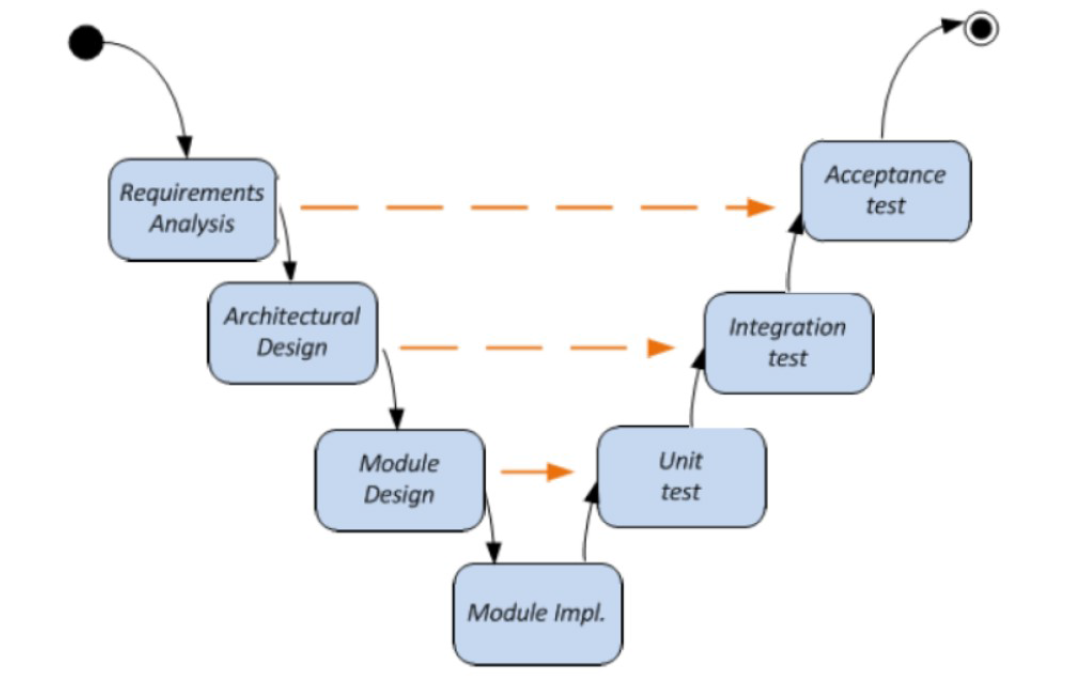
\includegraphics[width=1\textwidth]{Figurer/vmodel}
	\caption{V-modellen}
\end{figure}
På ovenstående figur ses V-modellen, hvor den første fase er udvikingen af kravspecifikationen. Hertil udvikles en tilhørende accepttest, som gør det muligt, at tjekke om systemet opfylder de stillede krav. Næste fase er systemarkitekturen, hvor der ligeledes udvikles en tilhørende test. Testen skal undersøge integrationen mellem de implementerede moduler. De to sidste faser er design og implementering, som der udføres løbende tests af. 

\subsection{Vandfaldsmodellen}
Vandfaldsmodellen er en model, der ofte benyttes for udviklingen af software. Udviklingen af software foregår på den måde, at en ny fase af modulen først påbegyndes, når den foranliggende fase er færdiggjort, som kan ses på figuren nedenfor. 
\begin{figure}[H]
	\centering
	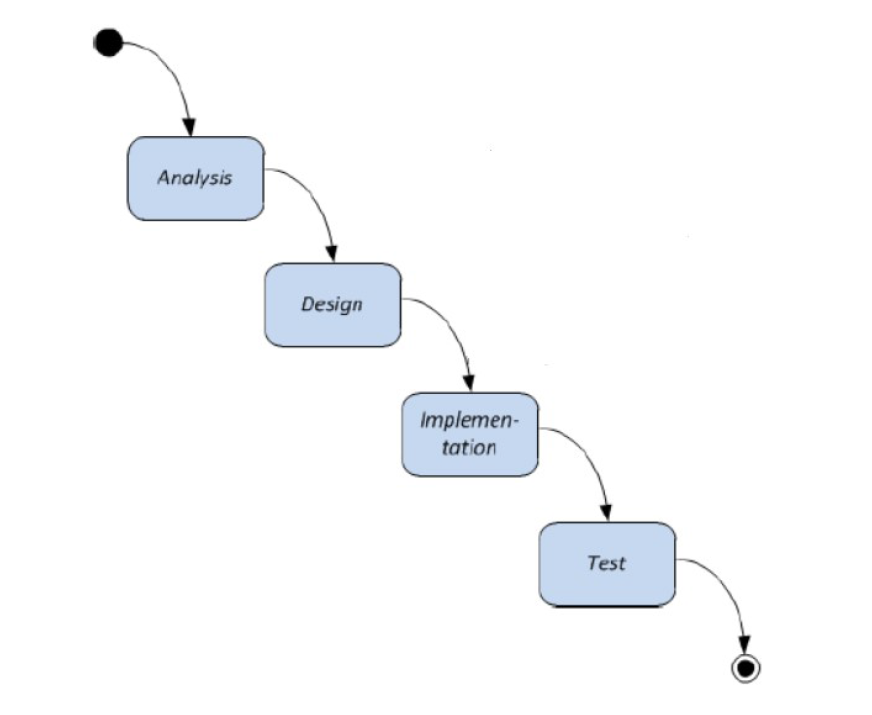
\includegraphics[width=0.8\textwidth]{Figurer/vfmodel}
	\caption{Vandfaldsmodellen}
\end{figure}
De tre udviklingsmodeller hænger alle sammen på den måde, at der arbejdes i kronologisk logisk rækkefølge. De har suppleret hinanden alle tre, hvor ASE-modellen har skabt det overordnede overblik. Vandfaldsmodellen er den udviklingsproces, som der er blevet arbejdet efter i alle projektets facetter. V-modellen har sikret, at de nødvendige tests af systemet og de enkelte moduler har fundet sted. 



\section{Metode}
Dette afsnit har til formål at beskrive hvilke metoder samt arbejdsredskaber, der er blevet benyttet til udarbejdelsen af software, hardware, rapport og dokumentation for projektet. 
\\\\
Der er blevet anvendt metoder samt viden fra forskellige kurser over 1.- 2.- og 3.semester. I kurset ST3KVI er der blevet benyttet viden om transducerprincippet samt generelt om blodtryksmåling, hvor der er i dette projekt fokuseres på den invasive blodtryksmåling. Fra kurserne ST2ITS2 og ST3ITS3 har viden om databasestruktur samt principperne om tre-lagsmodellen og Observer \& Stragety Pattern været grundlaget for opbygningen af softwaren. Et krav til projektet var, at der skulle kunne aktiveres og deaktiveres et digitalt filter. Til at designe dette filter blev der anvendt viden fra kurset E3DSB. Kurset ST1SUN1 har bidraget med viden om den anatomiske opbygning af hjertet samt blodtryk. Til beregning af komponentværdier, design og implementering af hardwaren er der blevet benyttet metoder og viden fra kurset E2ASB. Principperne om design diagrammer fra kurset I2ISE har bidraget til designafsnittet for hardware og software i dokumentationen. Alle kurserne har tilsammen været nødvendige for at kunne stå tilbage med dette specifkke produkt.
\\\\
Det er ud fra metoden SysML, software- og hardware design er blevet specificeret. Det er en metode, der anvender forskellige diagrammer til henholdsvis at beskrive softwarens opbygning og kommunikation samt hardwarens. Selve systemet vil også via SysML diagrammer blive beskrevet. Hensigten er at give læseren det store overblik over, hvilke aktør, der intergerer med systemet samt hvilken funktionalitet der tillægges systemet.
\\ \\
Softwaren er også beskrevet gennem metoden UML, helt specifikt ved et UML klassediagram. Klassediagrammet viser, hvilke klasser og metoder al softwaren består af, samt hvordan systemet er bygget op efter tre-lagsmodellen.
\\\\
For at forstå det grundlæggende om blodtryk og blodtryksmåling er der blevet anvendt en redegørende metode, hvor der er blevet indsamlet viden gennem læsning af sundheds- og tekniskfaglige børger samt hjemmesider. Ud fra den viden har det været muligt, at redegøre for principperne samt analysere de resultater systemet har givet.
\\\\
Efter hardwarens funktionalitet var bestemt blev der benyttet den matematiske metode til at beregne de forskellige komponentværdier, der skulle til for at realisere den ønskede hardware.

\subsubsection{Arbejdsredskaber} 
Af benyttede arbejdsredskaber er der først og fremmest brugt en fælles arbejdsplatform, GitHub. GitHub er en online platform, hvor der er mulighed for at foretage ændringer samtidigt, og gemme i en fælles mappe. Yderligere er der mulighed for en detaljeret versionshistorik.\\
Alle SysML- og UML-diagrammer er udarbejdet i programmet Visio. Koden er skrevet i sproget C\# i programmet Visual Studio. Visual Studio spiller også sammen med programmet WaveForms Generator, i forbindelse med simulering af blodtrykssignalet. Selve rapporten, mødereferater, logbog og dokumentationen er udformet i tekstprogrammet LaTex. MatLab, som er et signalbehandlingsprogram samt matematikprogram, der er blevet benyttet til at udarbejdelse af hardwaren. Yderligere er Facebook brugt til mødeindkaldelse og generel kommunikation.




\section{Specifikation og analyse}
\subsection{Hardware}


\section{Arkitektur}
\subsection{Design}
\subsection{Implementering og test af SW}
\subsection{Implementering og test af HW}

\section{Resultater og diskussion}

\section{Opnåede erfaringer}

\section{Fremtidigt arbejde}


